\documentclass[12pt]{article}
\usepackage{graphicx}
\usepackage{siunitx}
\usepackage{authblk}
\usepackage{amsmath}
\usepackage{booktabs} % for much better looking tables
\usepackage{array} % for better arrays (eg matrices) in maths
\usepackage{verbatim} % adds environment for commenting out blocks of text & for better verbatim
\usepackage{hyperref}
\usepackage[table,xcdraw]{xcolor}
\usepackage{url}
\usepackage[parfill]{parskip}
\usepackage[top=1in, bottom=1in, left=0.9in, right=0.9in]{geometry}
\geometry{letterpaper}
\usepackage{mathptmx}
\usepackage{lineno}
\linenumbers
\usepackage{afterpage}
\usepackage[T1]{fontenc}
\usepackage{amsmath}
\numberwithin{equation}{section}
% \usepackage[numbers]{natbib}
% \usepackage{fancyvrb}
%\usepackage{lineno}
\usepackage{cleveref}
\usepackage{xr}
\usepackage{natbib}
\bibliographystyle{abbrvnat}
\setcitestyle{authoryear,open={(},close={)}}
\usepackage{ccaption}% http://ctan.org/pkg/ccaption
\usepackage[labelfont=bf]{caption}

\makeatletter
\newcommand*{\addFileDependency}[1]{% argument=file name and extension
  \typeout{(#1)}
  \@addtofilelist{#1}
  \IfFileExists{#1}{}{\typeout{No file #1.}}
}
\makeatother

\newcommand*{\myexternaldocument}[1]{%
    \externaldocument{#1}%
    \addFileDependency{#1.tex}%
    \addFileDependency{#1.aux}%
}

\myexternaldocument{supplemental-info}

\title{A scalable and automated pipeline for the recovery of eukaryotic MAGs}
\author[1,*]{Harriet Alexander}
\author[2]{Sarah K. Hu}
\author[1]{Maria Pachiadaki}
\author[1,3]{Arianna I. Krinos}
\author[4]{Benjamin J. Tully}
\author[4]{Chris J. Neely}
\author[5]{Taylor Reiter}

\affil[1]{\small{Biology Department, Woods Hole Oceanographic Institution, Woods Hole, MA, USA}}
\affil[2]{Marine Chemistry and Geochemistry, Woods Hole Oceanographic Institution, Woods Hole, MA, USA}
\affil[3]{MIT-WHOI Joint Program in Oceanography, Cambridge and Woods Hole, MA, 02540}
\affil[4]{Department of Biological Sciences, University of Southern California, Los Angeles, CA 90089}
\affil[5]{Population Health and Reproduction, University of California, Davis, Davis, CA, 95616}
\affil[*]{Correspondence; halexander@whoi.edu}

\date{}

\begin{document}

\maketitle

\section*{Abstract}

\section*{Introduction}

Microbial eukaryotes, or protists, play a critical part in all ecosystems found on the planet. In addition to their vast morphological diversity, protists exhibit a range of functional roles and trophic strategies \citep{Caron2011Marine}. Protists are centrally important to global biogeochemical cycles, enabling carbon and nutrient flow [citations]. Despite their importance across ecosystems and in the global carbon cycle, research on microbial eukaryotes typically lags behind that of bacteria and archaea \citep{Caron2009Hypotheses, Keeling2017Marine}. Consequently, fundamental questions surrounding microbial eukaryotic ecological function remain unresolved. Novel approaches that enable genome retrieval from environmental -omic data will provide a means of bridging that knowledge gap. 

Binning,  or the process of reconstructing likely genomic units (genomes) or bins, draws associations between assembled genetic fragments (contigs) from metagenome based on a factors such as abundance and tetranucleotide frequency \citep{Alneberg2014Binning, Wu2014MaxBin, Kang_2019, Graham2017BinSanity}. Through a series of refinement steps, these bins can be honed to generate metagenome assembled genomes or MAGs \citep{Parks2017Recovery, Delmont2018Nitrogen-fixing, Tully2018reconstruction, Almeida2019new}. Binning metagenomic data into MAGs has revolutionized how researchers ask questions about microbial communities and has enabled the identification of novel taxa and functional traits \citep{Rinke2019phylogenomic, Tully2019Metabolic}. The lack of focus on eukaryotic MAGs is arguably twofold: (1) eukaryotic genomic complexity \citep{Zhang2011practical}, complicates both metagenome assembly and MAG retrieval; and (2) there is a bias in currently available metagenomic computational tools towards the study of bacterial and archaeal members of the community. Yet, much can be learned about the diversity and role of eukaryotes in our environment from eukaryotic MAG retrieval \citep{Olm2019Genome-resolved}.

Here we developed and applied EUKHeist, a scalable and reproducible pipeline to facilitate the retrieval, taxonomic assignment, and annotation of prokaryotic and eukaryotic metagenome assembled genomes (MAGs) from mixed community metagenomes. We applied this pipeline to metagenomic data from the Tara expedition protist-size fractions samples \citep{Carradec2018global}, encompassing more than 20Tb of raw sequence data. From these large-size fraction metagenomic samples, we recovered over 4,000 prokaryotic MAGs and 900 eukaryotic MAGs. 

\section*{Results and Discussion}
\subsection*{Prokayrotic MAGs recovered distinct from previous marine MAG efforts}



% Please add the following required packages to your document preamble:
% \usepackage[table,xcdraw]{xcolor}
% If you use beamer only pass "xcolor=table" option, i.e. \documentclass[xcolor=table]{beamer}

\begin{figure}[h!]    
    \centering
    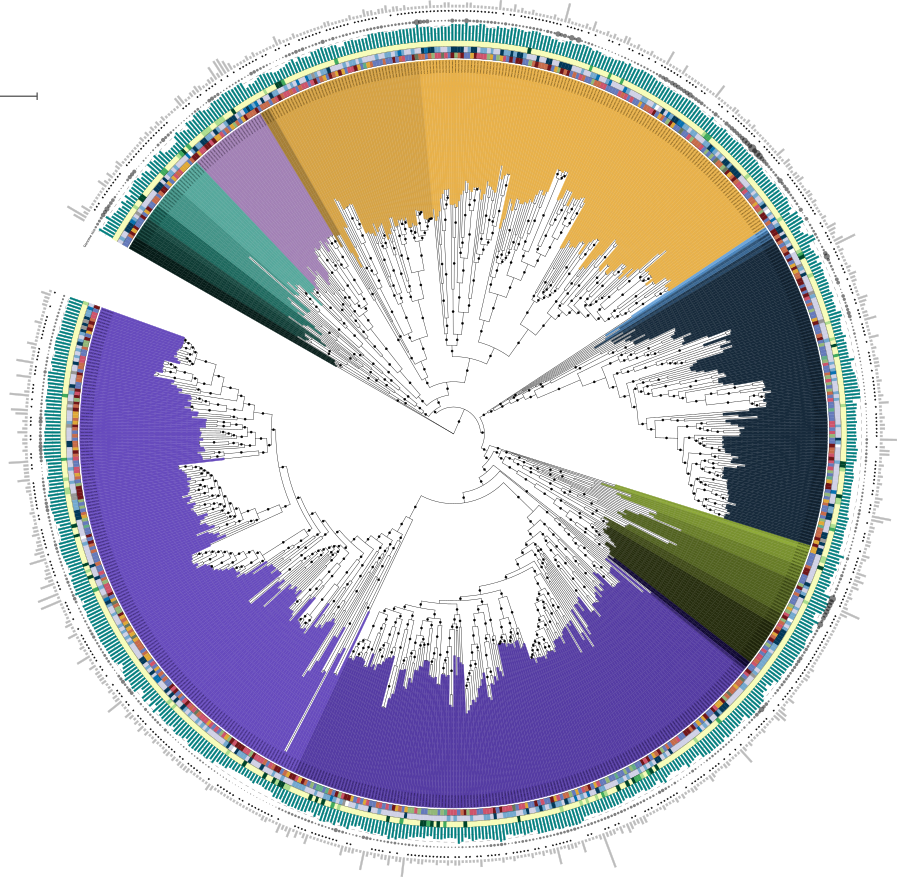
\includegraphics[width = 0.95\columnwidth]{figures/Figure1-prok-mags.png}
    \caption{\textbf{Diversity of the high-quality prokaryotic TOPAZ MAGs.} }
    \label{fig:fig4-trophy}
\end{figure}


\begin{table}[]
\caption{\textbf{Phyogenetic diversity and gain of various MAGs originating from Tara Oceans.} Phylogenetic divesrity and gain of proaryotic MAGs was assessed for this study (TOPAZ), TOBG \citep{Tully2018reconstruction}, UBA \citep{Parks2017Recovery}, and TARA \citep{Delmont2018Nitrogen-fixing}.}
\centering
\begin{tabular}{|
>{\columncolor[HTML]{EFEFEF}}c |c|c|c|c|}
\hline
{\color[HTML]{000000} \textbf{Base tree}}                  & \cellcolor[HTML]{EFEFEF}\textbf{\begin{tabular}[c]{@{}c@{}}MAG \\ designation\end{tabular}} & \cellcolor[HTML]{EFEFEF}\textbf{\begin{tabular}[c]{@{}c@{}}No. of added \\ MAGs\end{tabular}} & \cellcolor[HTML]{EFEFEF}\textbf{\begin{tabular}[c]{@{}c@{}}Phylogenetic \\ diversity* \end{tabular}} & \cellcolor[HTML]{EFEFEF}\textbf{\begin{tabular}[c]{@{}c@{}}Phylogenetic \\ gain\textdegree \end{tabular}} \\ \hline
{\color[HTML]{000000} \textbf{Neutral}} & TOPAZ (MQ, NR) & 1,571            & 59.9\%  & 42.8\%            \\ \hline
{\color[HTML]{000000} \textbf{Neutral}} & TOPAZ (HQ, NR) & 634              & 41.6\%  & 25.8\%            \\ \hline
{\color[HTML]{000000} \textbf{Neutral}} &   TOBG     & 1,974            & 61.3\%  & 46.7\%            \\ \hline
{\color[HTML]{000000} \textbf{Neutral}} & UBA            & 1,052            & 40.5\%  & 25.8\%            \\ \hline
{\color[HTML]{000000} \textbf{Neutral}} & TARA           & 722              & 44.4\%  & 31.0\%            \\ \hline
{\color[HTML]{000000} \textbf{Neutral}} & TOBG + UBA + TARA               & 3,750            & 66.6\%  & 51.8\%            \\ \hline
{\color[HTML]{000000} \textbf{\begin{tabular}[c]{@{}c@{}}Neutral + TOBG \\ + UBA + TARA\end{tabular}}}  & TOPAZ (MQ, NR) & 1,572            & 44.7\%  & 14.4\%            \\ \hline
{\color[HTML]{000000} \textbf{\begin{tabular}[c]{@{}c@{}}Neutral + TOBG \\ + UBA + TARA\end{tabular}}}  & TOPAZ (HQ, NR) & 634              & 26.1\%  & 6.2\%             \\ \hline
{\color[HTML]{000000} \textbf{\begin{tabular}[c]{@{}c@{}}Neutral + TOPAZ \\ + UBA + TARA\end{tabular}}} & TOBG           & 1,977            & 48.5\%  & 11.1\%            \\ \hline
{\color[HTML]{000000} \textbf{\begin{tabular}[c]{@{}c@{}}Neutral + TOPAZ\\ + TOBG + UBA\end{tabular}}}  & UBA            & 1,055            & 23.8\%  & 1.6\%             \\ \hline
{\color[HTML]{000000} \textbf{\begin{tabular}[c]{@{}c@{}}Neutral + TOPAZ\\ + TOBG + TARA\end{tabular}}} & TARA           & 722              & 28.0\%  & 3.4\%             \\ \hline
\multicolumn{5}{l}{\begin{tabular}[c]{@{}l@{}}\textbf{*} total branch length spanned by a set of taxa\\ \textbf{\textdegree} additional branch length contributed by a set of taxa
\end{tabular}}                
\end{tabular}
\label{tab:mags}
\end{table}

\subsection*{Eukaryotic genome recovery from metagenomes covers major \\ eukaryotic supergroups}
Our classification pipeline that identified putative eukaryotic bins of interest based on length ($>2.5$ Mbp) and proportion of base pairs that were predicted to be eukaryotic in origin by EukRep yielded 993 MAGs for further study (\Cref{fig:recovered}). Following protein prediction with taxonomy-informed EukMetaSanity (CITATION), the likely taxonomic assignment of these bins was made with MMSeqs taxonomy \citep{Steinegger2018} and EUKulele \citep{Krinos2021EUKulele}. 988 bins were found to annotate as likely eukaryotic bins based on the predicted protein homology consensus aligning with eukaryotic lineages (Supplemental Dataset 2). Of the 988 Eukyarotic MAGs recovered, 713 MAGs were estimated to be more than 10\% complete based on presence of core eukaryotic BUSCOs. For the purposes of our subsequent analyses, we consider MAGs that were greater than 30\% complete as (n=485) (\Cref{fig:fig3-euk}). 

A concatenated gene tree of the TOPAZ eukaryotic MAGs shows good reconstruction relative to protein-consensus based taxonomic annotation (\Cref{fig:fig3-euk}). The recovered MAGs spanned 8 major eukaryotic super groups: Archaeplastida (Chlorophyta), Opisthokonta (Metazoa, Choanoflagellata, and Fungi), Amoebazoa, Apusozoa, Haptista (Haptophyta), Cryptista (Cryptophyta), and the TSAR supergroup (Stramenopila and Aveolata) \citep{Burki_2020}. Taxonomic trends were observed for MAGs recovered from the various co-assemblies based on ocean region, depth, and size fraction. The highest diversity of MAGs were recovered from the small size fraction ($0.8-5 \mu m$), with MAGs recovered from all major groups list above (\Cref{fig:all-dist}). Additionally, the smallest size fraction yielded most eukaryotic MAGs (n=311) recovered (\Cref{fig:fig3-euk,fig:all-dist}). Of the MAGs recovered in the smallest size fraction,  Chlorophyta (n=133), SAR (n=56), and Orchophyta (n=57) were best represented. There were fewer eukaryotic MAGs recovered from the other size fraction groups $5-20\mu m$ (n=20), $20-180 \mu m$ (n=87), and $180-2000\mu m$ (n=39) (\Cref{fig:all-dist}). Within each of these groups, metazoan constituted the most recovered MAGs, representing $>80\%$ of recovered MAGs in the two largest size fractions. MAGs were also recovered from all discrete sampling depths (SRF (n=315), DCM (n=133), MES (n=13)) as well as samples where no discrete depth was sampled (MIX n=21) and the filtered seawater controls, FSW (n=3), including 1 chlorophyta MAG (TOPAZ\_IOF1\_E003) which was estimated to be 100\% complete with no contamination (Supplemental Dataset 2). A total of 16 highly complete fungal MAGs were recovered in this project, of those, 11 were recovered from the MES (\Cref{fig:fig3-euk,fig:hq-dist}), of all but one MAG were attributed to Ascomycota, with one being attributed to Basidiomycota aligning with previous molecular taxonomic estimates \citep{Morales_2019,Pernice_2015,Edgcomb_2010}. Deep-sea fungi have been found to have functional profiles that are enriched for the metabolism of secondary metabolites, vitamins (e.g. vitamin B5), and amino acids \citep{Morales_2019,DAMARE2006172} 

Eukaryotic MAGs were recovered from across all ocean regions surveyed, with the largest number of high quality eukaryotic MAGs recovered from the South Pacific Ocean Region (SPO) (n=143) with the fewest recovered MAGs were from the Southern Ocean (SO) (n=11) and Red Sea (RS) (n=12) (\Cref{fig:hq-dist}). These trends appear to align well with the overall sequencing depth at each of these location (Supplemental Dataset 1). Unlike depth and size fraction, there was no bias observed in the taxonomic composition of MAGs across ocean regions (\Cref{fig:all-dist,fig:hq-dist}). 

Globally, fungal MAGs had the highest overall average completeness ($87 \pm 15\%$) and metazoan MAGs had the lowest ($50 \pm 13\%$) (\Cref{fig:all-prot-bar,fig:hq-prot-bar}). Fungi (12.5 - 47.8Mb). Putative fungal TOPAZ MAGs were recovered from the phyla Ascomycota and Basidiomycota which have average genome sizes of 36.9 and 46.5 Mb, respectively \citep{Mohanta_2015}. The average size of recovered metazoan MAGs was 43.2 Mb (6.5-177Mbp), encompassing an average of 14600 proteins (\Cref{fig:hq-prot-bar}). 76 of the 123 metazoan MAGs we recovered here were likely Hexanauplia (Copepoda). Copepods have been estimated to be up to 2.5 Gb with high variation (10-fold difference) across sequenced members \citep{Jorgensen_2019}.  

Chlorphyta MAGs were smaller and had fewer predicted proteins than other eukaryotic MAGs despite demonstrating comparable completeness metrics, with an average MAG size of 13.9 Mbp and 7525 predicted proteins (\Cref{fig:hq-prot-bar}). By contrast, Cryptophyta and Haptophya had the largest average MAG size with 50.8 Mbp and 44.4 Mbp with an average of 23500 and 24400 predicted proteins, respectively.

% \afterpage{\clearpage}
\begin{figure}[h!]    
    \centering
    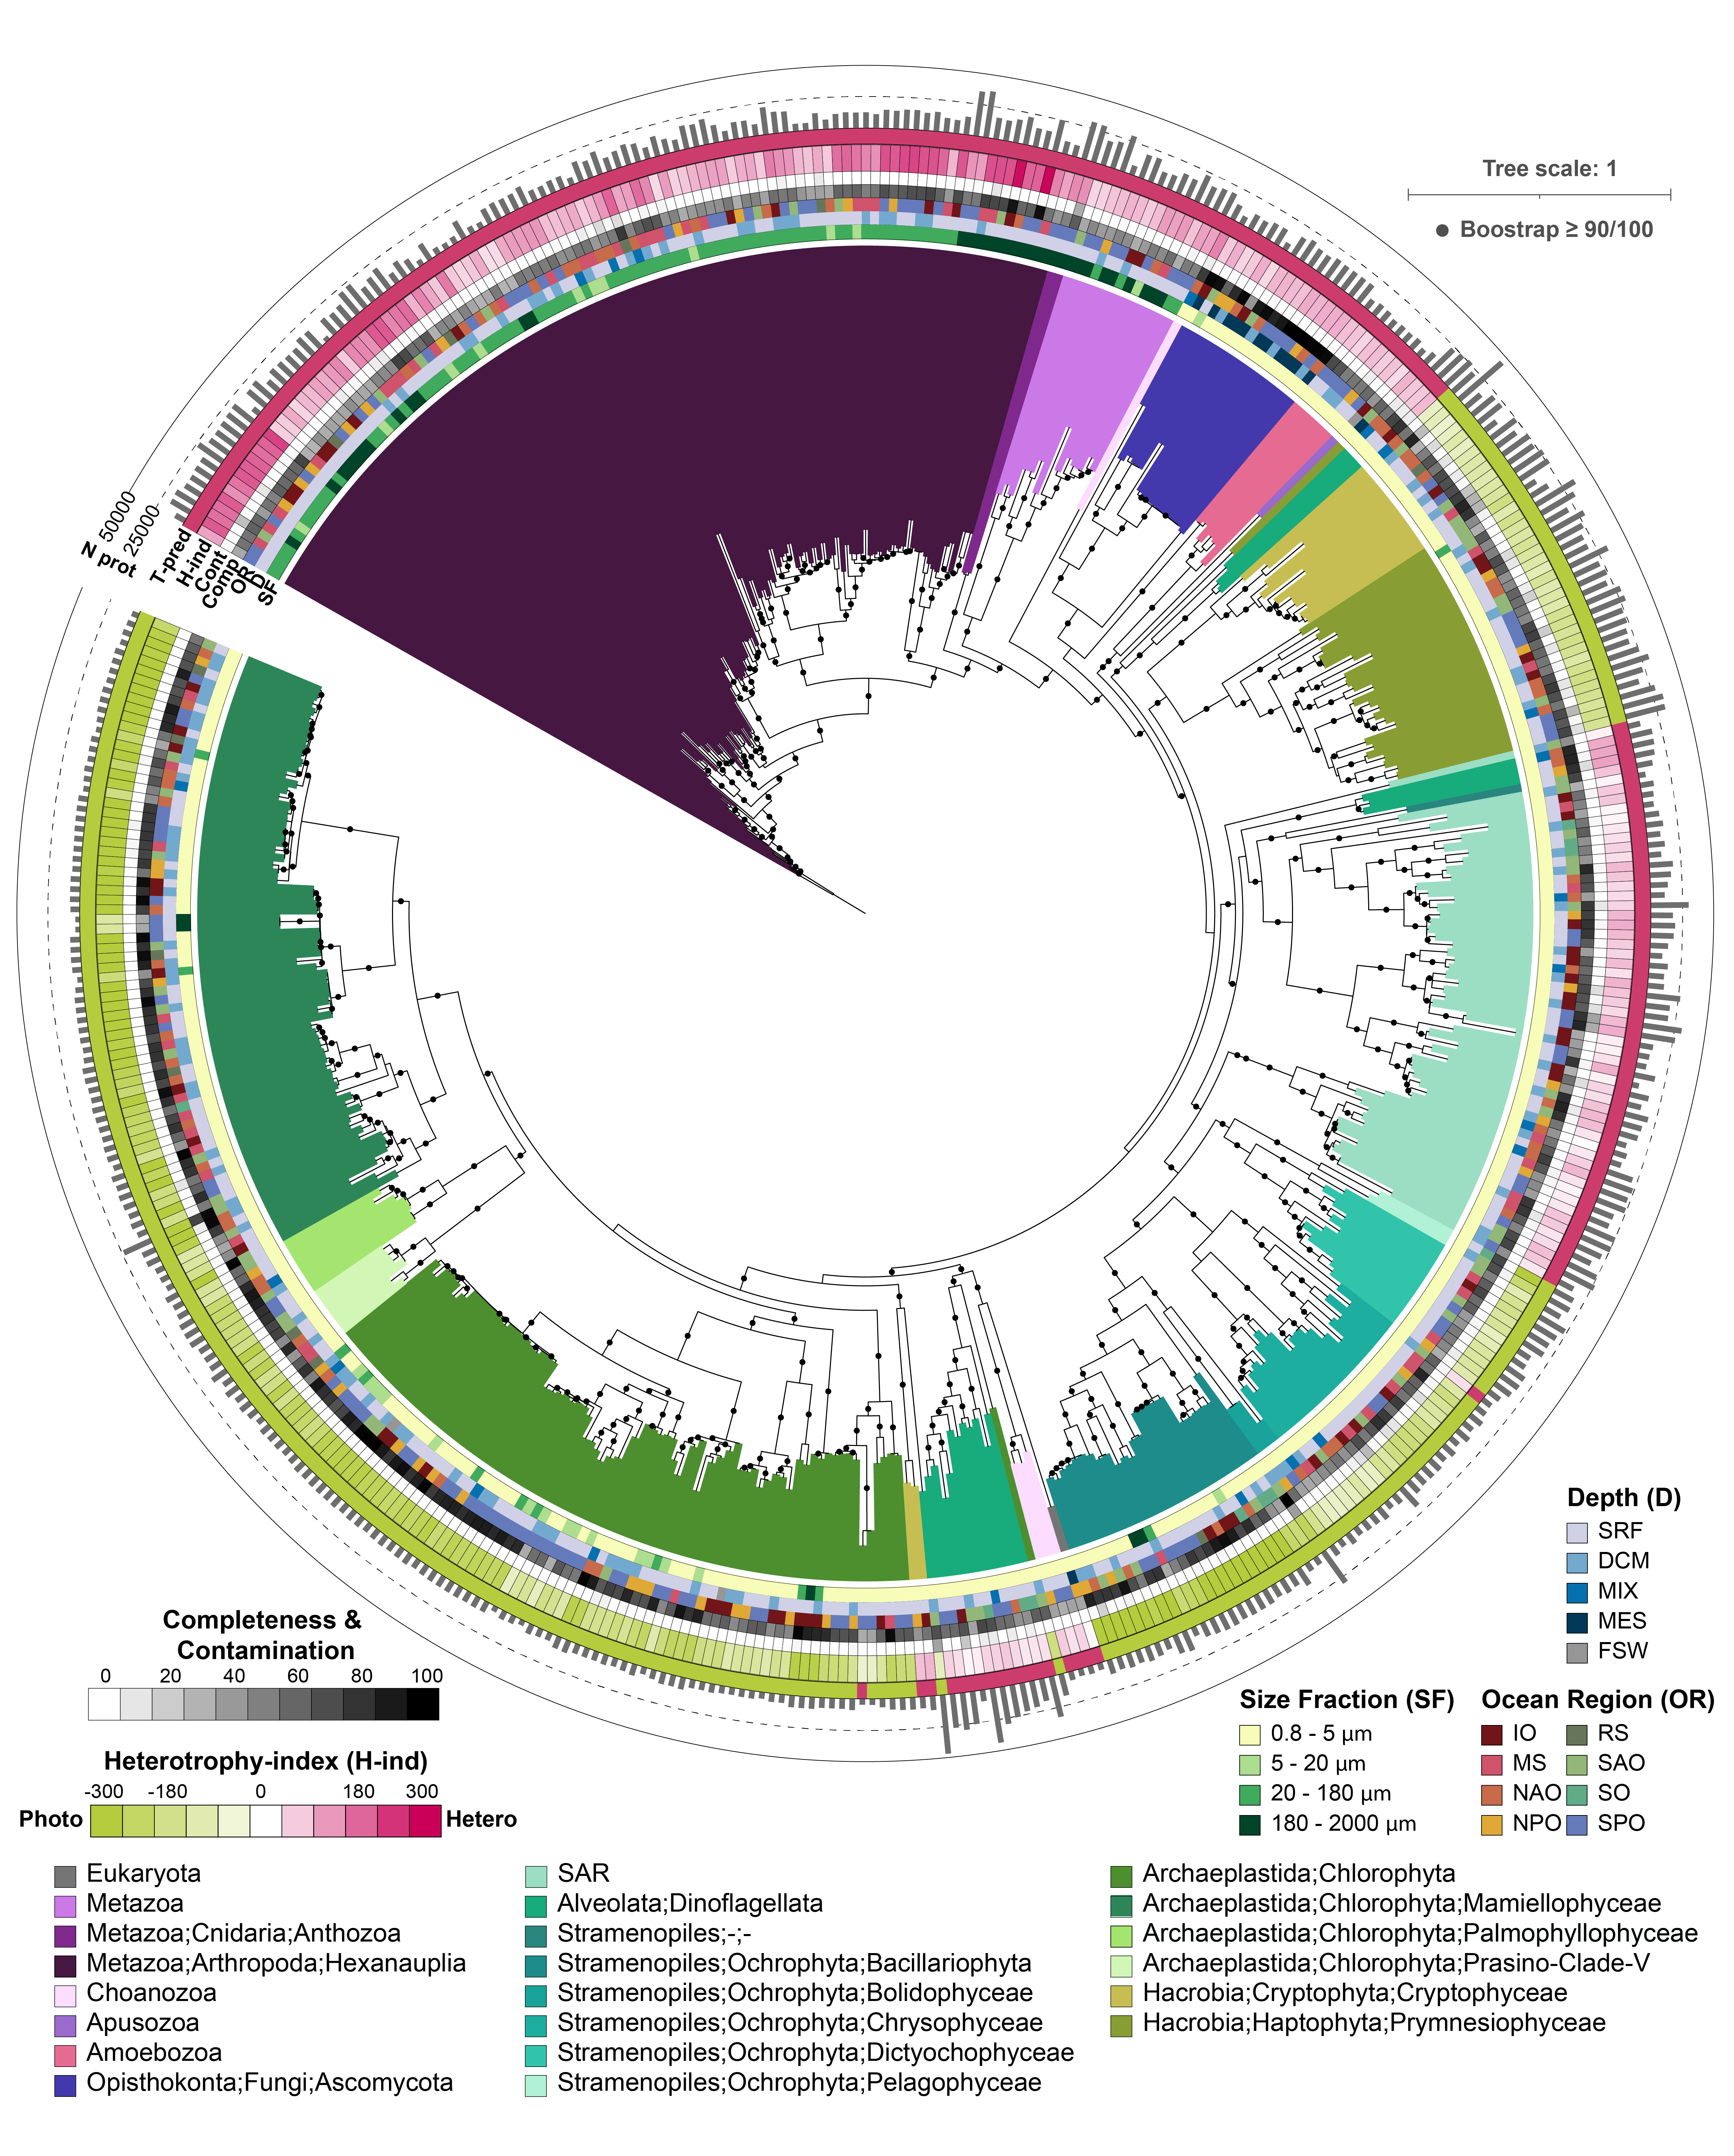
\includegraphics[width = \columnwidth]{figures/Figure3_EukPhylogeny_30Busco-v2-01.png}
    \caption{[Continued on next page.]}
    \label{fig:fig3-euk}
\end{figure}
\begin{figure}[t]
  \contcaption{\textbf{TOPAZ eukaryotic MAGs span the eukaryotic tree of life.} The maximum likelihood tree was inferred from a concatenated protein alignment of 49 proteins from the eukaryotic BUSCO gene set that were found to be commonly present across at least 75\% of the 485 TOPAZ eukaryotic MAGs that were estimated to be >30\% complete based on BUSCO ortholog presence. Branches (nodes) are colored based on consensus protein annotation estimated by EUKulele and MMSeqs. The Ocean Region (OR), Depth (D), and Size Fraction (SF) of the co-assembly that a MAG was isolated from is color coded as colored bars. The completeness (comp) and contamination (cont) as estimated based on BUSCO presence are depicted as a heatmap. Predicted heterotrophy-index (H-ind), which ranges from phototroph-like (-300) to heterotroph-like (300) is shown as a heatmap. The predicted trophic mode (T-pred) based on the trophy random forest classifier with heterotroph (pink) and phototroph (green), is depicted. The number of proteins predicted with EukMetaSanity are shown as a bar graph along the outermost ring. }% Continued caption
\end{figure}
The taxonomic patterns of MAG recovery aligned well with the trends observed in the relative abundance of MAGs across samples. Metazoan MAGs dominated the larger size fractions ($20-180 \mu m$ and $180-2000 \mu m$) across both the surface and DCM across stations, while chlorophyta MAGs were dominant across most of the small size fraction stations ($0.8-5 \mu m$). A notable exception are the stations from the Southern Ocean where Haptophyta and Ochrophyta were most abundant in all size fractions. Compared to the pelagic samples, SRF and DCM, the average recruitment of reads from the MES recruited to the Eukaryotic MAGs was far lower ($24500 \pm 34450$ average TPM in the MES compared to $131000 \pm 104000 $ and $136000 \pm 85000$ for the SRF and DCM, respectively). This suggests that the mesopelagic have high variability across communities \citep{Pernice_2015} and that we did not fully capture the eukaryotic MAGs that adequately describe all surveyed communities. Alternatively, this might suggest that the communities sampled were dominated by prokaryotic community members \citep{Pernice_2014}.  

%Maybe move to SI text? 
The relative abundance of eukaryotic MAGs across samples was correlated with environmental parameters (\Cref{fig:ind-corr}) and were found to broadly cluster by course taxonomic grouping, as such abundances were summed across were summed by course taxonomic group to assess  \Cref{fig:env-corr}) to assess general trends and correlations in patterns of abundance. Globally, we note that metazoan MAG abundance significantly (Bonferroni corrected $p<0.001$) positively correlated with temperature, salinity, and retention time (defined as the average length of time that a particle has been trapped in an eddy), and significantly negatively correlated with a variety of nutrients (phosphate, nitrate+nitrite, silica), CDOM, and depth (meaning they are more abundant in surface samples). This suggests that the metazoan MAGs we are recovering are likely abundant in the subtropical and tropical waters of the large ocean gyres that are oligotrophic. Notably, Choanozoa and Amoebazoa clustered with Metazoans, forming a distinct cluster from other more typically photosynthetic and planktonic groups. Chlorophyta, Apusozoa, Cryptophyta, Dinoflagellata, Ochrophyta, SAR, and Haptophyta clusterd separately from Metazoa and were typified by significant positive correlation with oxygen, \textit{a}, and nitrite (\Cref{fig:env-corr}). Additionally, MAGs recovered that belonged to Ochrophyta were found to be significantly negatively correlated with temperature. This suggests that these MAGs were likely associated with more polar or subpolar regions.


\subsection*{Trophic mode can be predicted from MAG gene content}

Using a reference set built from expression data, we predicted the trophic mode the complete MAGs using machine learning and direct estimation via presence of important KEGG pathways. Accordingly, we have predicted both a broad trophic category and a quantitative extent of heterotrophy for each MAG. These predictions aligned exceptionally well with the putative taxonomy of each MAG, and illuminated important patterns with respect to the global distribution of these trophic strategies. Further, our data-driven trophic mode predictions correlate well with an independent model designed to identify the presence of photosynthetic machinery and capacity for phagotrophy \citep{burns2018gene}.

An important note is that, as of present, the references are only derived from expression-level data. While this means that important genes related to trophic strategy may be missed from the prediction workflow, this is also exciting, because it means that there is much room for growth for these already skillful predictions. As genomic references become available and the number of transcriptomic experiments continue to grow, we can expect to further constrain the classes of genes that decide trophic mode. Additionally, we used the entire MMETSP and EukProt databases with manually assigned trophic strategies, which includes several with dubious annotations, or that might have been from an experiment that influenced its expressed trophic mode. This is especially important for mixotrophs, which may act more like heterotrophs or phototrophs in alignment with culture conditions. As databases grow, they could be pruned to include only experiments in which the trophy of the organism was known exactly, which would enable the patterns of expression which decide trophic mode to be  pinpointed more precisely. Ideally, a core set of protein families necessary for heterotrophy and for phototrophs could be identified, and mixotrophy could be characterized by the proportion of these sets which overlap in the genome or the expression profile of the candidate organism.

\begin{figure}[h!]    
    \centering
    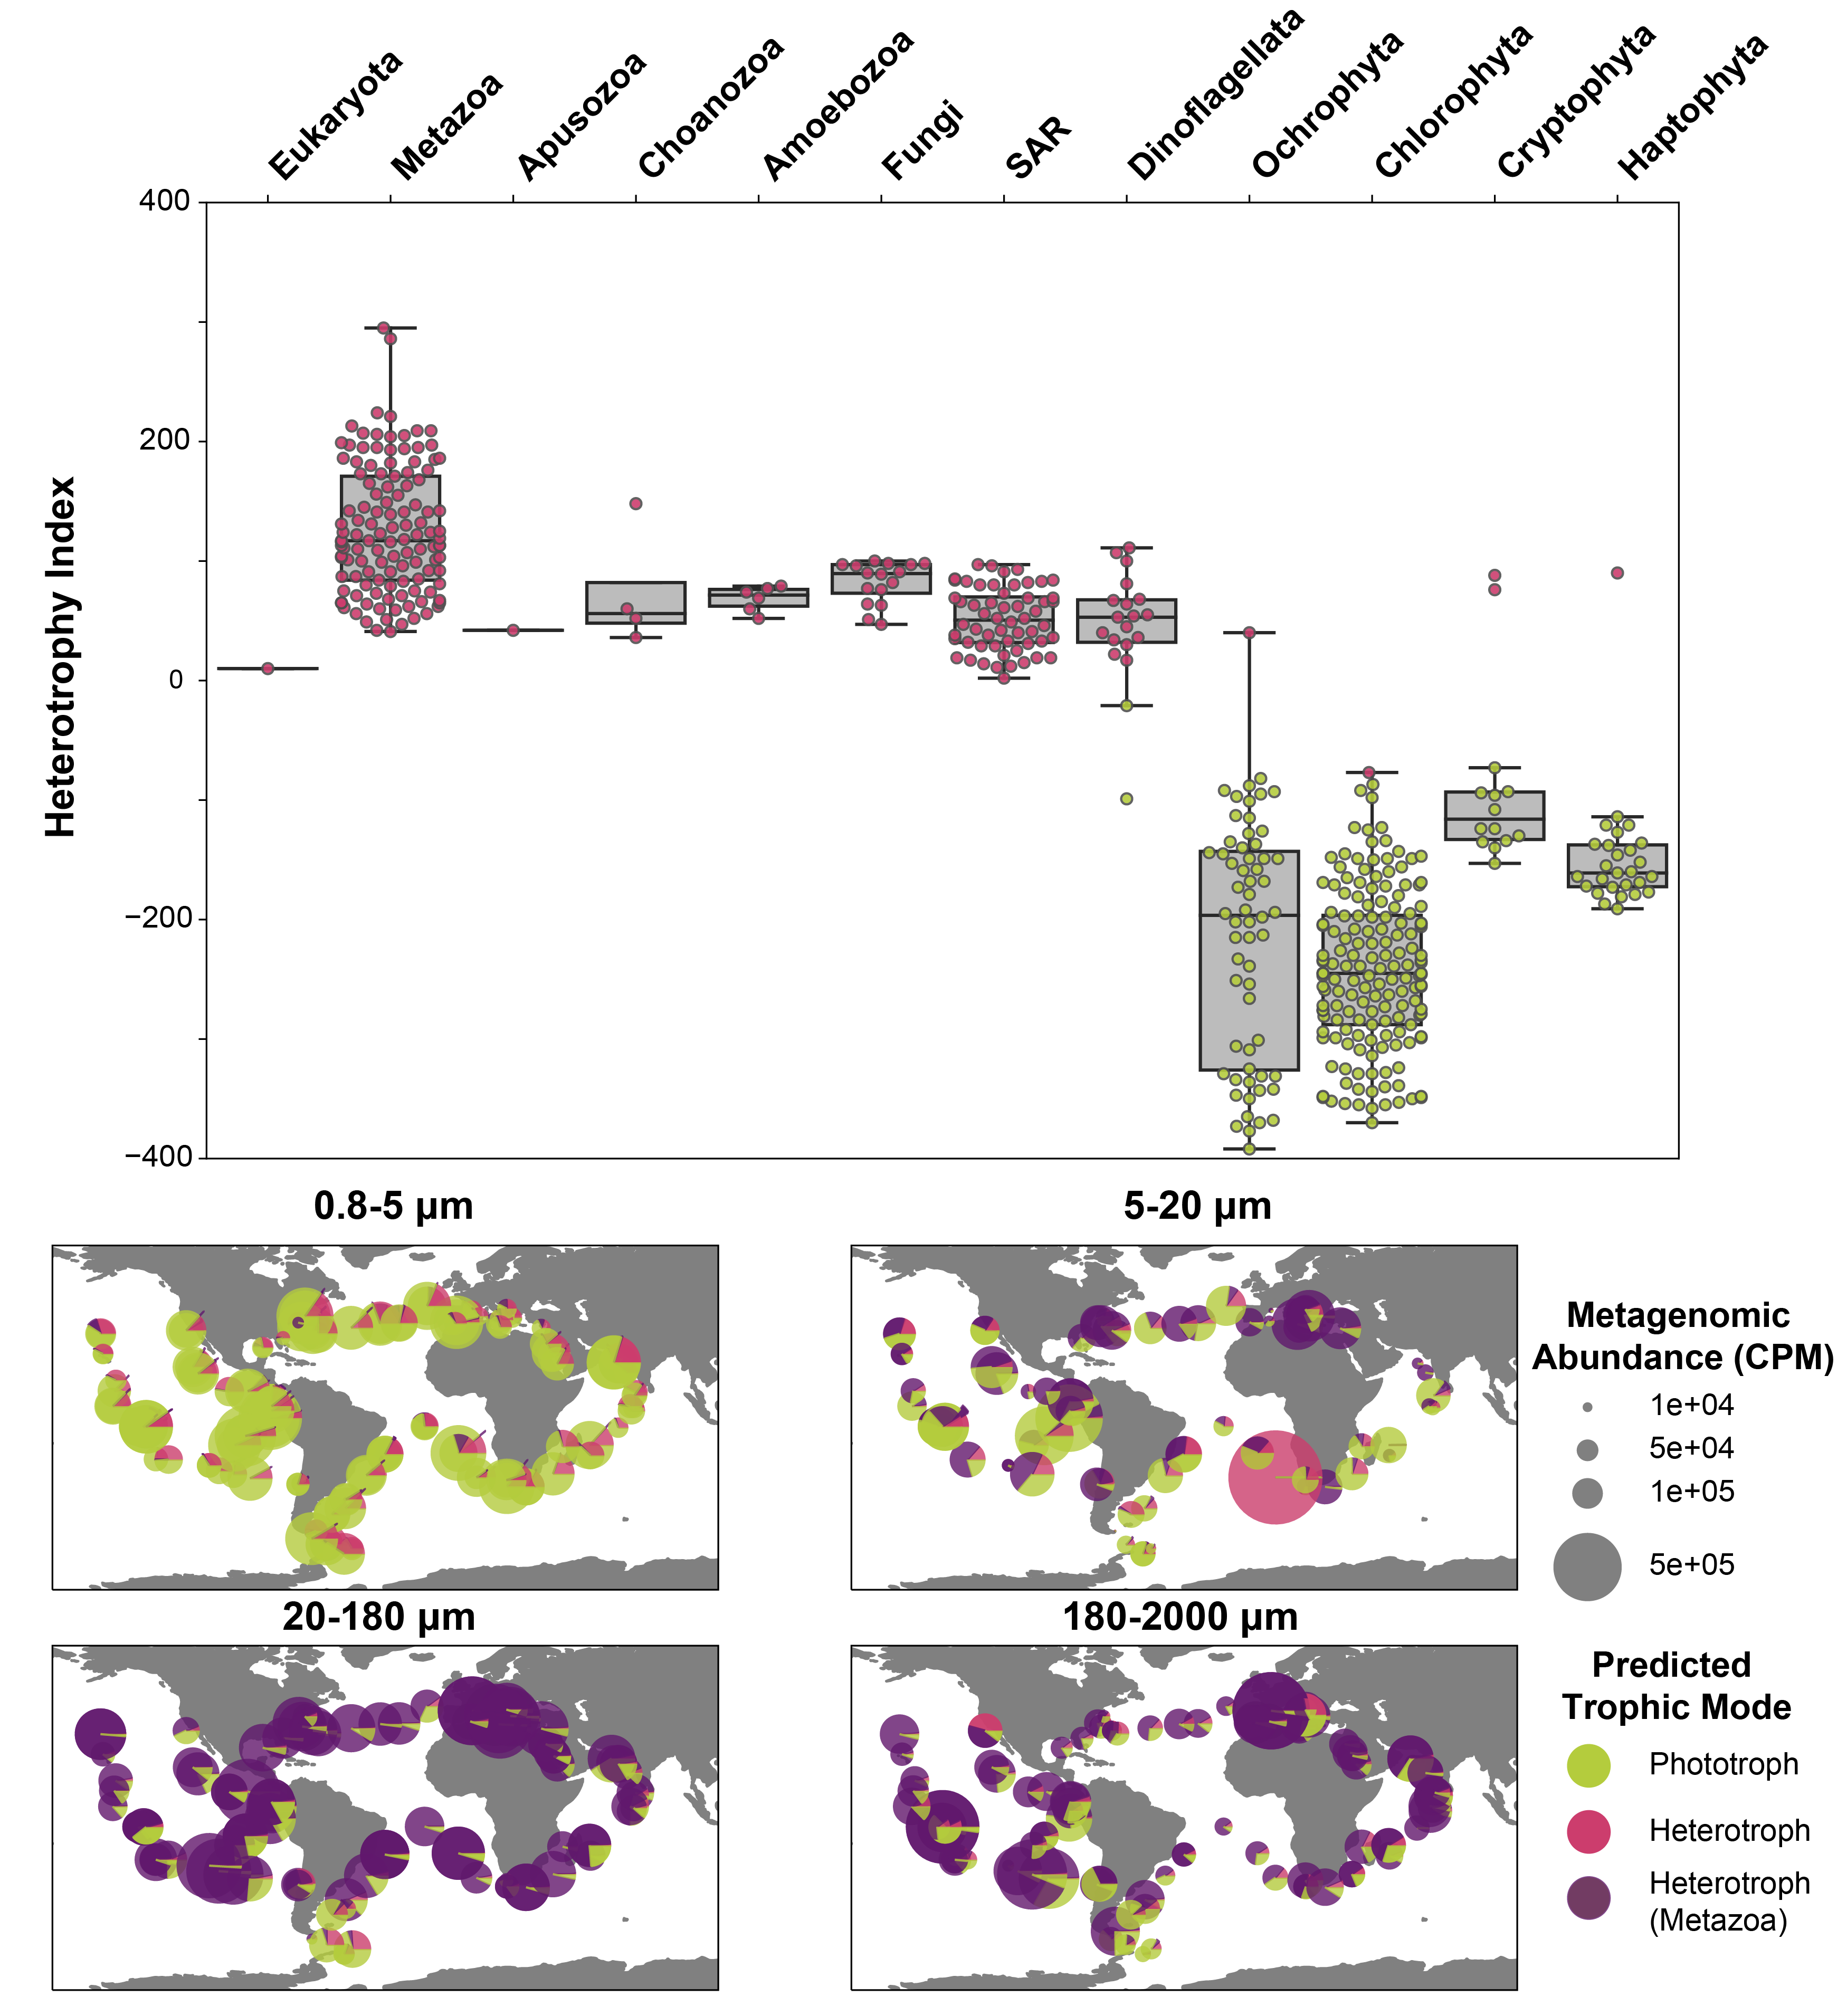
\includegraphics[width = 0.9\columnwidth]{figures/Figure4_Trophic_Mode_v2-01.png}
    \caption{\textbf{Estimated trophic status of TOPAZ eukaryotic MAGs.} (Top) Trophic status was predicted for each high-completion TOPAZ eukaryotic MAG using a Random Forest model trained on the presence and absence of KEGG orthologs and is shown as a color (green, phototroph, pink, heterotroph). The Heterotrophy Index (\cref{eq:hind})  for each MAG is plotted with a box plot showing the range of the H-index for each higher level group. (Bottom) The relative distribution and abundance of Phototroph (green), non-Metazoan Heterotroph (Pink), and Metazoan Heterotroph (Purple) is depicted across all surface samples. Plots are subdivided by size classes. }
    \label{fig:fig4-trophy}
\end{figure}

\subsection*{Metatranscriptomic evidence highlights ecological niches of SAR and Dicyochophyte MAGs}

\begin{figure}[h!]    
    \centering
    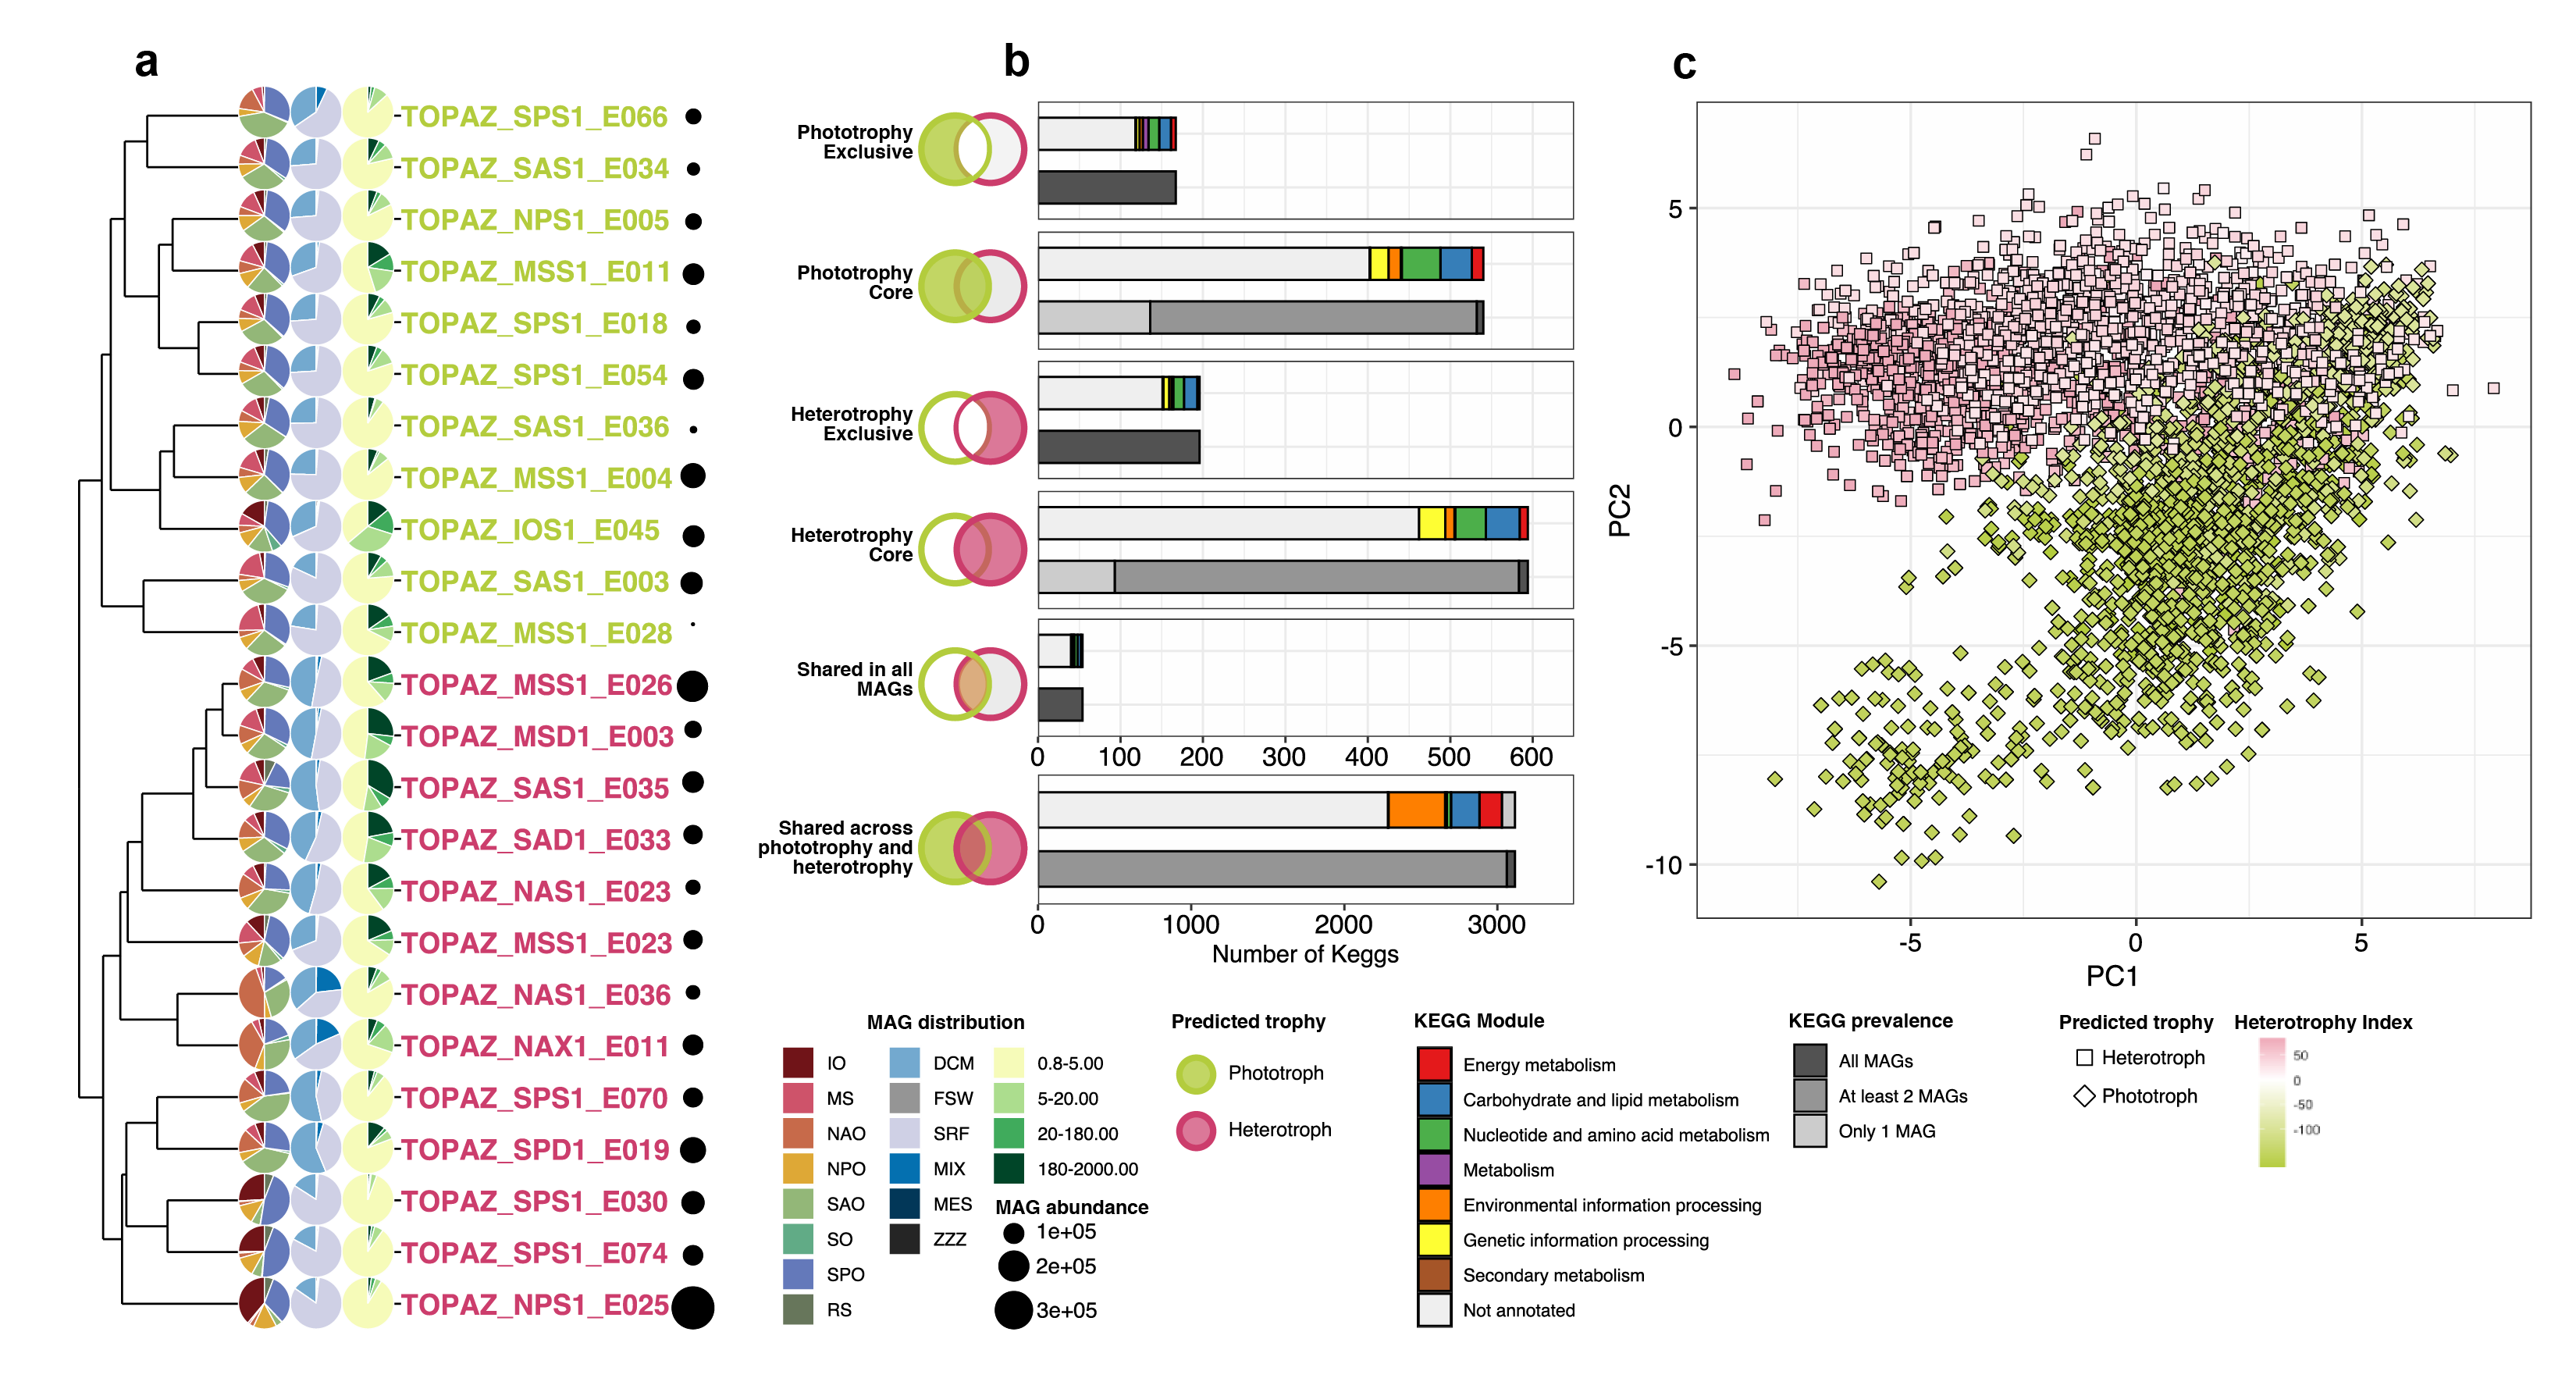
\includegraphics[width = \columnwidth]{figures/Figure5-dendro-dictyo-panels-01.png}
    \caption{ \textbf{Dictyochophyte + Stramenopile MAGs} }
    \label{fig:fig5-dicty}
\end{figure}


\subsection*{Co-occurring MAGs structured by environmental factors } %might we call them guilds? 

\begin{figure}[h!]    %Place holder figure for right now. 
    \centering
    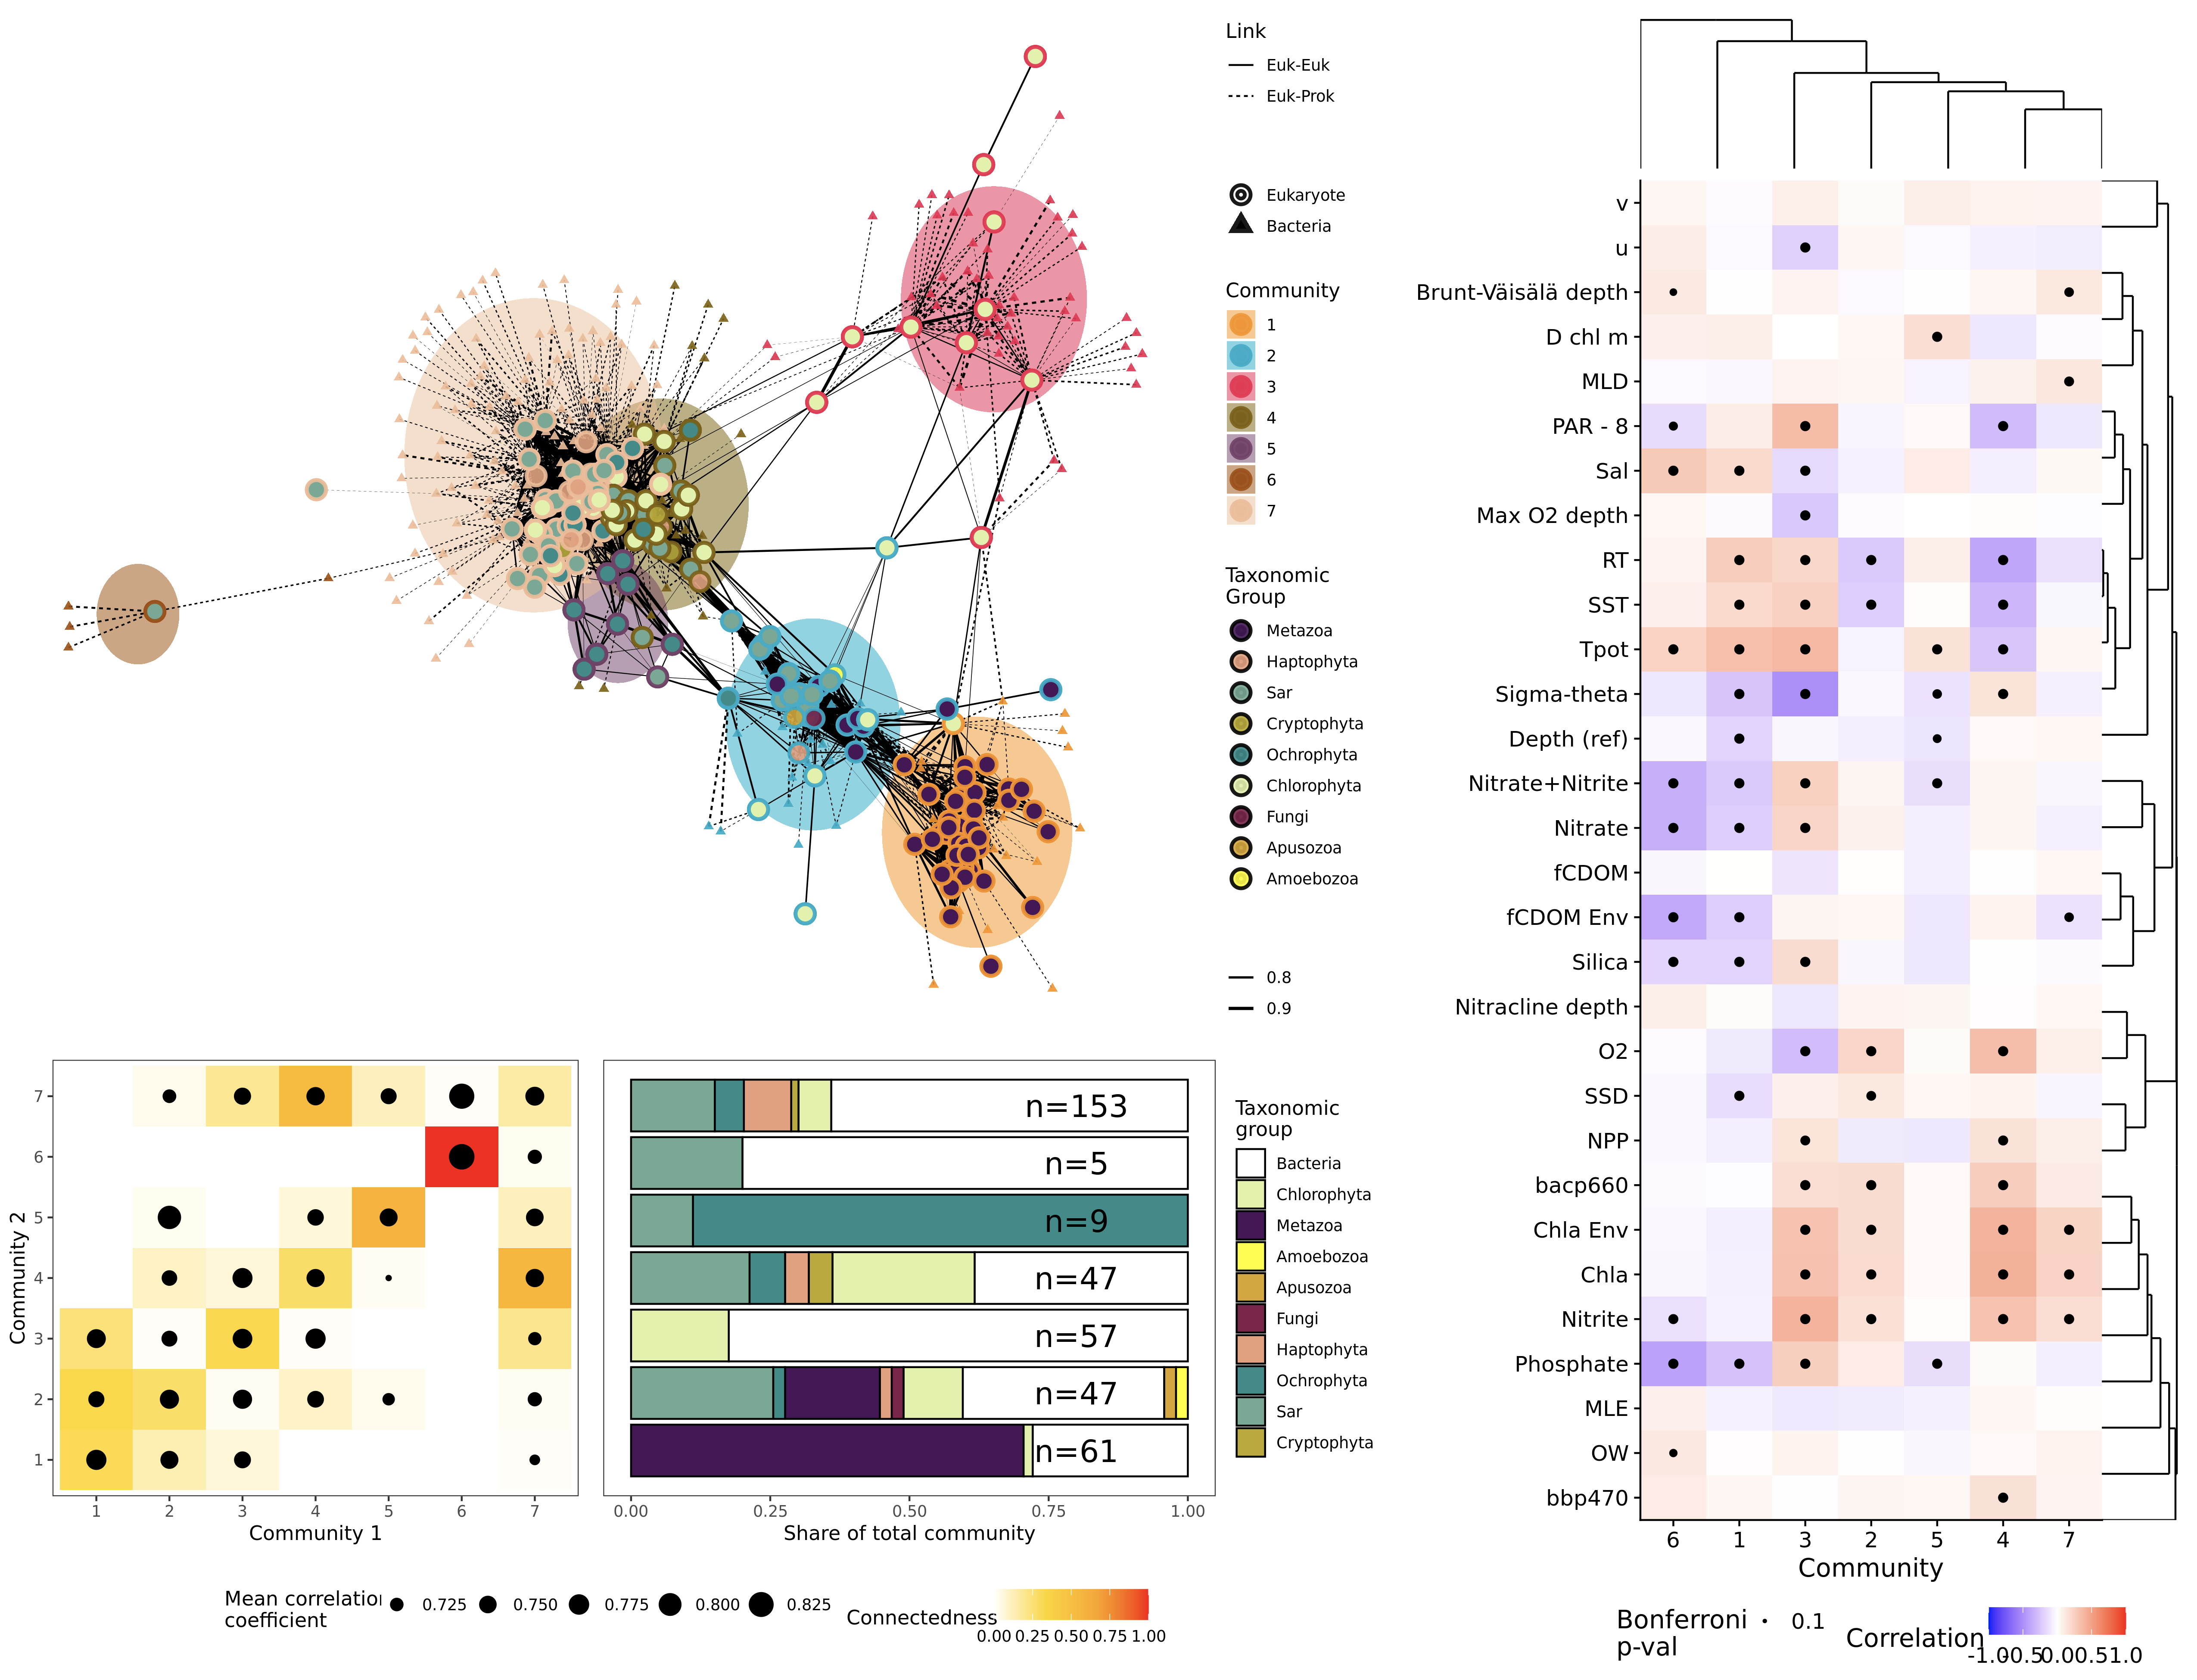
\includegraphics[width = \columnwidth]{figures/Figure6_Networks.png}
    \caption{ \textbf{Distinct communities recovered from the TOPAZ MAGs.} Network analysis performed on association of eukaryotic MAGs with one another and the bacterial MAGs resulted in the identification of seven communities. These communities showed distinct patterns of taxonomic composition (panel B) and were uniquely correlated to environmental parameters (panel C).}
    \label{fig:fig4-trophy}
\end{figure}


\section*{Conclusion}
\section*{Materials and Methods}

\subsection*{Data acquisition} The metagenomic and metatranscriptomic data corresponding to the size fractions dominated by eukaryotic organisms ranging from microbial eukaryotes and zooplankton ($0.8 -  2000 \mu m$) as originally published by \citet{Carradec2018global} were retrieved from European Molecular Biology Laboratory-European Bioinformatics Institute (EMBL-EBI) under the accession numbers PRJEB4352 (large size fraction metagenomic data) and PRJEB6603 (large size fraction metatranscriptomic data) on November 20, 2018. Only samples with paired end reads (forward and reverse) were used in the subsequent analyses (Supplementary Table ERR numbers and input files). After an initial sample-to-sample comparison with sourmash (SI figure sourmash), it was determined that samples largely clustered by depth and size fraction. Samples were grouped for co-assembly by size fraction ($0.8 - 5 \mu m$, $5-20 \mu m$, $20-180 \mu m$, and $180-2000 \mu m$) as per \citet{Carradec2018global}, depth or sample type (surface (SRF), deep chlorophyll maximum (DCM), mesopelagic (MES), mixed surface sample (MIX), and filtered seawater (FSW)), and geographic location (Supplementary Table X). In cases where a sample did not fall directly within one of the size classes, it was assigned to an existing size class based on the upper um limit of the sample. This grouping resulted in the combination of 824 cleaned, paired FASTQ files samples into 94 distinct co-assembly groups, which were used downstream for co-assembly (assembly stats Table X). 

\subsection*{EUKHeist pipeline for metagenome assembly and binning}The metagenomic analysis, assembly, binning, and all associated quality control steps were carried out with a bioinformatic pipeline, EUKHeist, that enables user-guided analysis of stand-alone metagenomic or paired metagenomic and metatranscriptomic sequence data. EUKHeist is a streamlined and scalable pipeline currently based on the Snakemake workflow engine \citep{Koster2012} that is configured to facilitate deployment on local HPC systems.  Supplemental Figure X outlines the structure and outputs of the existing EUKHeist pipeline. EUKHeist is designed to retrieve and identify both eukaryotic and prokaryotic MAGs from large, metagenomic and metatranscriptomic datasets (Supplementary Figure Pipeline). EUKHeist takes input of sequence meta-data, user-specified assembly pairings (co-assembly groups) (Supplementary Table X), and raw sequence files, and returns MAGs that are characterized as either likely eukaryotic or prokaryotic. 

Here, all raw sequences accessed from the EMBL-EBI were quality assessed with FastQC and MultiQC \citep{Andrews2010FastQC}. Sequences were trimmed using Trimmomatic (v. 0.36; parameters: \texttt{ILLUMINACLIP: 2:30:7, LEADING:2, TRAILING:2, SLIDINGWINDOW:4:2, MINLEN:50}) \citep{Bolger2014Trimmomatic}. Passing mate paired reads were maintained for assembly and downstream analyses. Quality trimmed reads co-assembled assembled based on the assembly groups (Supplementary table X) with MEGAHIT (v1.1.3, parameters: \texttt{k= 29,39,59,79,99,119}) \citep{Li2015MEGAHIT}. Basic statistics were assessed for all assemblies with Quast (v. 5.0.2) \citep{Gurevich_2013} (Supplementary Table Y). Cleaned reads from assembly-group-associated metagenomic and metatranscriptomic samples were mapped back against the assemblies with bwa mem (v.0.7.17) \citep{Li2010Fast}. The bwa-derived abundances were summarized with MetaBat2 (v. 2.12.1) script \texttt{jgi\_summarize\_bam\_cotig\_depths} (with default parameters). The output contig abundance tables were used along with tetranucleotide frequencies to associate contigs into putative genomic bins using MetaBat2 (v. 2.12.1) \citep{Kang_2019}. The Snakemake profile used to conduct this analysis is available at \url{https://www.github.com/alexanderlabwhoi/tara-euk-metag}. A generalized version of the Snakemake pipeline (called EUKHeist) that might be readily applied to other datasets is available at \url{https://www.github.com/alexanderlabwhoi/EUKHeist}. MAGs here are subsequently named and referred to as Tara Oceans Partial Associated MAGs (TOPAZ) and are individually named based on their assembly group (SI Table Assembly Group naming)

\subsection*{Identification of putative Eukaryotic MAGs} The binning process described above recovered a total of 16,385 putative bins. These bins were screened to identify high completion eukaryotic and prokaryotic bins. All bins were first screened for length, assuming that eukaryotic bins would likely be greater than 2.5Mbp in size (modeled off of the size of the smallest known eukaryotic genome, $\sim 2.3$Mbp \textit{Microsporidian Encephalitozoon intestinalis} \citep{Corradi2010complete}). Bins larger than 2.5Mbp were screened for relative eukaryotic content using EukRep \citep{West2018Genome-reconstruction}, a k-mer based strategy that estimates the likely domain-origin of metagenomic contigs. EukRep was used to classify the relative proportion of eukaryotic and prokaryotic content in each bin in a contig-by-contig manner. This approach identified 907 candidate eukaryotic bins that were greater than 2.5Mb in length and estimated to have more than 90\% eukaryotic content by length. Protein coding domains were predicted in all 907 putative eukaryotic bins using EukMetaSanity. 

\subsection*{Protein prediction in Eukaryotic MAGs with EukMetaSanity} 
\paragraph{Taxonomy.} The MMseqs2 v12.113e3 \citep{Steinegger2017, Steinegger2018, Mirdita2019} \texttt{taxonomy} module (parameters: \texttt{-s 7 --min-seq-id 0.40 -c 0.3 --cov-mode 0}) was used to provide a first-pass taxonomic assignment of the input MAG for use in a downstream element of EukMetaSanity pipeline that requires an input NCBI taxon id or a taxonomic level (i.e. Order, Family, etc.). We created a custom database comprising both OrthoDB \citep{Kriventseva2018} and MMETSP \citep{Keeling2014} protein databases (OrthoDB-MMETSP) that integrates NCBI taxon ids. MMseqs2 was used to query each MAG against the OrthoDB-MMETSP database to identify a first-pass taxonomic assignment. The lowest common ancestor of top scoring hits was identified to provide taxonomic assignment to each candidate eukaryotic bin. The \texttt{taxonomyreport} module generates a taxon tree that includes the percent of MMseqs mappings that correspond to each taxonomic level. A taxonomic identifier and scientific name are selected to the strain level or when total mapping exceeds 8\%, whichever comes first. The assigned NCBI taxon id is retained for downstream analyses. 

\paragraph{Repeats identification.} RepeatModeler \citep{Flynn-RM, RepeatModeler} was used to provide \textit{ab initio} prediction of transposable elements, including short and long interspersed nuclear repeats, as well as other DNA transposons, small RNA, and satellite repeats. RepeatMasker \citep{RepeatMasker} was then used to hard-mask these identified regions, as well as any Family-level (as identified above) repeats from the DFam 3.2 database \citep{Flynn2020}. RepeatMasker commands \texttt{ProcessRepeats} (parameter: \texttt{-nolow}) and \texttt{rmOutToGff3} (parameter: \texttt{-nolow}) were used to output masked sequences (excluding low-complexity repeat DNA from the mask) as FASTA and gene-finding format (GFF3) files, respectively. 

\paragraph{\textit{Ab initio} prediction.}  GeneMark \citep{Lomsadze2005} was used to generate \textit{ab initio} gene predictions with the repeat-masked eukaryotic candidate bin sequences output from the prior step. The GeneMark subprogram ProtHint attempts to use Order-level proteins from OrthoDB-MMETSP database to generate intron splice-site predictions for \textit{ab initio} modeling using GeneMark EP  \citep{Bruna2020}. If ProtHint fails to generate predictions, then GeneMark will default to ES mode. Due to the fragmented nature of metagenomic assemblies, the prediction parameter stringency was drastically reduced relative to what is recommended for draft genome projects (parameters: \texttt{--min\_contig 500 --min\_contig\_in\_predict 500 --min\_gene\_in\_predict 100}). These parameters can be easily modified within the EukMetaSanity config file. GeneMark outputs predictions of protein coding sequences (CDS) and exon/intron structure as GFF3 files. 


\paragraph{Integrating protein evidence.} MetaEuk \citep{LevyKarin2020} was used to directly map the repeat-masked eukaryotic candidate bins sequences against proteins from the OrthoDB-MMETSP database. MetaEuk \texttt{easy-predict} (parameters: \texttt{--min-length 30 --metaeuk-eval 0.0001 -s 7 --cov-mode 0 -c 0.3 -e 100 --max-overlap 0}) used Order-level proteins to identify putative CDS and exon/intron structure. MetaEuk encodes this output as headers in FASTA sequences that are then parsed into GFF3 files. 

\paragraph{Merging final results.} GFF3 output from the previous \textit{ab initio} and MetaEuk protein evidence steps were input into Gffread \citep{Pertea2020} (parameters: \texttt{-G --merge}) to localize predictions from both lines of evidence into a single GFF3 output file.  Each locus was then merged together using an  Python \citep{Python} script and the BioPython API \citep{BioPython} within EukMetaSanity. The set of \textit{ab initio} generated exons in each locus is used as a prediction of the underlying exon/intron structure of the gene locus to which it is assigned. If there are any protein-evidence-generated exons present at the same locus, and if the total numbers of exons predicted by each line of evidence have $\geq 70\%$ agreement, \textit{ab initio} generated exons lacking a corresponding protein-evidence-generated exon are removed (the first and last exon(s) of a locus are not removed). Conversely, any protein-evidence-generated exon present that lacks a corresponding \textit{ab initio} generated exon is added to the predicted exon/intron structure. The final gene structure for each locus is then processed into GFF3 and FASTA format.

\subsection*{Functional and taxonomic annotation of eukaryotic MAGs} 

Predicted proteins from EukMetaSanity were annotated for function against protein families in Pfam with PfamScan \citep{Finn2014Pfam} and KEGG using kofamscan \citep{Kanehisa_2019, Aramaki_2019}. The relative completeness and contamination  of each putative Eukaryotic MAG was assessed based on protein content using BUSCO v 4.0.5 against the eukaryota\_odb10 gene set using default parameters \citep{Simao2015BUSCO} and EukCC v 0.2 using the EukCC database created on 10/22/2019 \citep{Saary2020Estimating}. Annotation and completeness assessment were carried out using a EukHeist-Annotate (\url{https://www.github.com/halexand/Eukheist-annotate}).EukCC \citep{Saary2020Estimating} was also used to calculate MAG completeness and contamination. The average completeness across groups increased in all cases with EukCC except for metazoans, which on average had a lower estimated completeness (\Cref{fig:eukcc}). 

The taxonomic affiliation of the high- and low-completion bins was estimated using MMSeqs taxonomy through EukMetaSanity and EUKulele \citep{Krinos2021EUKulele}, an annotation tool that takes a protein-consensus approach, leveraging a Last Common Ancestor (LCA) estimation of protein taxonomy, as well as MMSeqs2 taxonomy module \citep{Steinegger2017, Steinegger2018, Mirdita2019}. Taxonomic level estimation in EUKulele was assessed based on e-value derived best-hits, where percent id was used as a means of assessing taxonomic level, with the following cutoffs: species, >95\%; genus, 95-80\%; family, 80-65\%; order, 65-50\%; class, 50-30\% modeled off of Carradec et al. (2018). All MAGs were searched against the MarMetZoan combining the MarRef, MMETSP, and metazoan orthoDB databases \citep{Johnson2018Re-assembly, Keeling2014, Kriventseva2018, Klemetsen:2017fg}. This databse is available for download through EUKulele. 

\subsection*{Phylogeny of eukaryotic MAGs} 
%A concatenated gene tree of the high-quality TOPAZ eukaryotic MAGs, the TARA MAGs (Delmont), and relevant select reference genomes and transcriptomes (MMETSP).
A total of 49 BUSCO proteins were found to be present across 80\% or more of the highly complete eukaryotic TOPAZ MAGs and were selected for the construction of the tree. Amino acid sequences from all genomes and transcriptomes of interest were collected and aligned individually using mafft (v7.471) (parameters: \texttt{--thread -8 –auto}) \citep{Katoh2013MAFFT}. Individual protein alignments were trimmed to remove sections of the alignment that were poorly aligned with trimAl (v1.4.rev15) (parameters: \texttt{-automated1}) \citep{Capella-Gutierrez2009trimAl}. Protein sequences were then concatenated and trimmed again with trimAl (parameters: \texttt{-automated1}). A final tree was then constructed using RAxML (v 8.2.12; parameters: \texttt{raxmlHPC-PTHREADS-SSE3 -T 16 -f a -m PROTGAMMAJTT -N 100 -p 42 -x 42}) \citep{Stamatakis2014RAxML}. The amino acid alignment and construction was controlled with a Snakemake workflow: \url{https://github.com/halexand/BUSCO-MAG-Phylogeny/}. Trees were visualized and finalized with iTOL \citep{Letunic2016Interactive}. 

\subsection*{Prokaryotic MAG assessment and analysis} 
The 15,478 bins that were not identified as putative eukaryotic bins based on length and EukRep metrics were screened to identify quality prokaryotic bins. The quality and phylogenetic-association of these bins was assessed with a modified version of MAGpy \citep{Stewart2019MAGpy}, which was altered to include taxonomic annotation with GTDB-TK \citep{Stewart2019MAGpy}. Bins were assessed based on single copy ortholog content with CheckM \citep{Parks2015CheckM} to identify 3 different bin quality sets: 1) high-quality prokaryotic bins (>90\% completeness, <5\% contamination), 2) medium-quality prokaryotic bins (90-75\% completeness, <2.5\% contamination), and 3) low-quality prokaryotic bins (75-50\% completeness, <2.5\% contamination). A total of 4022 prokaryotic MAGs met the above criteria. A final set of 2,407 non-redundant MAGs were identified using dRep v2.6.2 \citep{Olm_2017}, which performs pairwise genome comparisons in two steps. First, a rapid primary algorithm, Mash \citep{Ondov_2016} is applied. Genomes with Mash values equivalent to 90\% Average Nucleotide Identity (ANI) or higher were then compared with MUMmer \citep{Mar_ais_2018}. Genomes with ANI $\geq99\%$ were considered to belong to the same cluster. The best representative MAGs were selected based on the dRep default scoring equation \citep{Olm_2017}. Out of the final set of 2,407, 716 were high-quality MAGs. The same pipeline was used to determine the high-quality non-redundant MAGs reconstructed from the Tara Oceans metagenomes in previous studies \citep{Tully2018reconstruction, Parks2017Recovery, Delmont2018Nitrogen-fixing}. All MAGs were classified using GTDB-Tk v.0.3.2 \citep{Chaumeil_2019}.

\subsection*{Phylogeny of bacterial non-redundant high-quality MAGs}
Only 5 out of the 716 high-quality non-redundant MAGs were found to belong to Archeae, thus only bacterial MAGs were used for the construction of the phylogenetic tree with GToTree v.1.4.10 \citep{Lee_2019} and the gene set (HMM file) for Bacteria (74 targets). GToTree pipeline uses prodigal \citep{Hyatt_2010} to retrieve the coding sequences in the genomes, and HMMER3 \citep{Eddy_2011} to identify the target genes based on the provided HMM file. MUSCLE \citep{Edgar_2004} was then used for the gene alignments, and Trimal \citep{Capella_Gutierrez_2009} for trimming. The concatenated aligned is used for the tree constructions using FastTree . Three genomes were removed from the analysis due to having too few hits. The tree was visualized using iToL \citep{Letunic2016Interactive}.

\subsection*{Prokaryote MAG phylogeny comparison} 
A set of 8,644 microbial genomes were collected from the MarDB database \citep{Klemetsen:2017fg}(accessed 31 May 2018) encompassing the publicly available marine microbial genomes. Genomes were assessed using CheckM 
v1.1.1 \citep{Parks2015CheckM}(parameters: \texttt{lineage\_wf}) and genomes estimated to be <70\% complete or >10\% contamination were discarded. The remaining genomes (n = 5,878) were assessed using CompareM v0.0.23
(parameters: \texttt{aai\_wf}; \url{https://github.com/dparks1134/CompareM}) and near identical genomes were identified using a cutoff of $\geq 95\%$ average amino acid identity (AAI) with $\geq 85\%$ orthologous fraction (determined as one standard deviation from the average orthologous fraction for genomes with $97-100\%$ AAI).
Based on CheckM quality, the genome with the highest completion and/or lowest contamination were retained. From the remaining genomes (n = 3,843), all MAGs derived from the Tara Oceans dataset, specifically from Tully et al. \citet{Tully2018reconstruction} and Parks et al. \citet{Parks2017Recovery}, were removed. The remaining genomes (n = 2,275) would be used to form the base of a phylogenetic tree representing the available genome diversity prior to the release of previous Tara Oceans related MAG datasets \citet{Tully2018reconstruction, Parks2017Recovery, Delmont2018Nitrogen-fixing}, termed the ``neutral`` component of subsequent phylogenetic trees.

For the comparisons, phylogenetic trees were constructed using GToTree v1.4.7 \citep{Lee_2019} (default parameters; 25 Bacteria\_and\_Archaea markers). Any genome added to a tree that did not meet the default 50\% marker presence requirement was excluded from that tree. Five iterations of phylogenetic trees were constructed using the neutral genomes paired with each Tara Oceans MAG dataset, the high-quality TOPAZ prokaryote MAGs, and the medium-quality TOPAZ prokaryote MAGs, individually, and two larger trees were constructed containing all neutral genomes and Tara Oceans MAGs, with additions of either high- or medium-quality TOPAZ MAGs. Phylogenetic trees were assessed using genometreetk (parameter: \texttt{pd}; \url{https://github.com/dparks1134/GenomeTreeTk}) to determine the phylogenetic diversity (i.e., the total branch length traversed by a set of leaves) and phylogenetic gain (i.e., the additional branch length added by a set of leaves) \citep{Parks2017Recovery} for each set of MAGs compared against the neutral genomes and for the TOPAZ prokaryote MAGs compared against the neutral genomes and the other Tara Oceans MAGs.

\subsection*{MAG abundance profiling} 

Raw reads from all metagenomic and metatranscriptomic samples were mapped against the eukaryotic and prokaryotic TOPAZ MAGs to estimate relative abundances with CoverM (v. 0.5.0; parameters: \texttt{-min-read-percent-identity 0.95 -min-read-aligned-percent 0.75  -min-covered-fraction 0 -contig-end-exclusion 75 -trim-min 0.05 -trim-max 0.95  -proper-pairs-only}; \url{https://github.com/wwood/CoverM}). The total number of reads mapped to each MAG was then used to calculate Reads Per Kilobase Million ($RPKM$), where for some MAG, $i$ :  $RPKM_i = {X_i}/{l_iN}10^9$, with $X =$ total number of reads recruiting to a MAG, $l =$ length of MAG in Kb, $N =$ total number of trimmed reads mapping to a sample in millions. We also calculated transcripts per million (TPM), a normalization of the RPKM to the sum of all RPKMs in a sample. TPM was first proposed by Wagner et al. (Wagner:2012) \citep{Wagner_2012} as an alternative to RPKM that reduces statistical bias. The metric has since been applied to metagenomics data, sometimes called GPM (genes per million) \citep{Gradoville_2017}. 

\subsection*{Nutritional modelling} 

To predict the trophic mode of the high quality TOPAZ eukaryotic MAGs (n=485), a Random Forest model \citep{Breiman_2001} was constructed and calibrated using the ranger \citep{Wright_2017} and tuneRanger packages in R \citep{tuneRanger}, respectively. The model was trained using KEGG Orthology (KO) annotations \citep{Kanehisa_2019} from a manually-curated reference trophic mode transcriptomic dataset consisting of the MMETSP \citep{Keeling2014} and EukProt \citep{Richter2020EukProt}. 644 of the transcriptomes in this reference dataset came from the MMETSP (Keeling:2014), after 22 transcriptomes were removed due to low coverage of KEGG and Pfam annotations \citep{Finn2014Pfam}. The remaining XX came from the EukProt database, after XX were removed due to low compleness. Nutritional strategy (phototrophy, heterotrophy, or mixotrophy) was assessed for each reference transcriptome individually (citation?), 25\% of the combined reference transcriptomes were excluded from model training as testing data. 

A subset of KEGG Orthologs (KOs) that were predictive for trophic mode classification was determined computationally with the vita variable selection package in R \citep{Janitza_2016}, which was tested and justified by Degenhardt et al. \citet{Degenhardt_2017}. The model was built using these KOs with the 75\% of the combined database assigned as training data.

Additionally, we developed a secondary metric for assessing the extent of heterotrophy of a transcriptome or MAG. As opposed to the trinary classification scheme of the Random Forest model, this approach quantifies the extent of heterotrophic alignment. We calculate the likelihood of vita selected KOs used in the Random Forest model above to be present within heterotrophic, phototrophic, or mixotrophic reference transcriptomes. Three scores ($h$, $p$, $m$), one corresponding to each trophic mode, were hence calculated for each KO ($k$) (n=1000???). If  a given KO occurred in fewer than 50\% of the reference transcriptomes for a trophic mode, it was considered not to be characteristic of that trophic mode and as such the score was transformed ($-(0.5 - h),\ \text{if} \ h<0.5$), to reflect the absence. In the test transcriptome dataset, the transformed ratio-transformed scores were negated when a given KO was absent from the transcriptome. Hence, if for instance a KO was found in 10\% of reference transcriptomes assigned to heterotrophy, and absent in the reference transcriptome, it would receive a score of $-1 * (-(1-0.1)) = 0.9$ for that KO.

The scores for all KOs selected by vita were then used to scale the presence/absence patterns observed across transcriptomes and MAGs. Thus, for each transcriptome or MAG a single score was calcuated for each trophic mode heterotrophy ($H$), phototrophy ($P$), and mixotrophy ($M$) for all KOs present within the transcriptome or MAG ($K$):
  \begin{equation}\label{eq:sum}
  H = \sum_{k \in K} h_k \\ 
  \end{equation}
  \begin{equation}
    P = \sum_{k \in K} p_k \\
\end{equation}
  \begin{equation}
    M = \sum_{k \in K} m_k
\end{equation}

These calculated values can then be aggregated to a composite heterotrophy score ($H_{ind}$). The score was computed as follows: 
\begin{equation}\label{eq:hind}
   H_{ind}=
    \begin{cases}
      -1^{(H-P)}\sqrt{(H-P)^2}, & \text{if}\ M-max(H,P)<50, \\
      \frac{{}-1^{(H-P)}\sqrt{(H-P)^2}}{M}, & \text{if} \ M-max(H,P) \geq 50
    \end{cases}
  \end{equation}
  
\subsection*{Ecological analysis of SAR and Dicyochophyte MAGs}
24 high quality TOPAZ eukaryotic MAGs were selected due to phylogenetic placement in either the SAR group or Dictyochophyceae class. We saught to further interpret and investigate the physiological potential of these MAGs based on metatranscriptome profiling across Tara samples. 

For MAGs assigned to the Dictyochophyceae class, ASVs with a similar distribution were In addition to MAGs assigned to the Dictyochophyceae class using EUKulele, MAGs which had a similar distribution to Amplicon Sequence Variants (ASVs) or which the class assignment to Dictyochophyceae fell below the EUKulele default 50\%, were isolated as putative Dictyochophyceae MAGs. The relative abundance of Amplicon Sequence Variants (ASVs), derived from a sequence survey targeting the V9 hypervariable region, (cite de Vargas and Zenodo DOI from Callahan et al) was compared to the TPM relative abundances of MAGs. MAGs and ASVs were matched to one another based on similar taxonomic placement (i.e., equivalent division or class level assignment) and on sample co-occurrence (ASV and MAG had to appear in the same Tara survey sample). ASV and MAG pairs that co-occurred in at least 25 samples and the results of linear regression of ASV and MAG relative abundances had an $r^2 > 0.6$ were subset. Functions to compare 18S rRNA gene ASV and MAG relative abundances are available (https://shu251.github.io/dictyochophyceae-analysis/). %Putative dictyochophyceae MAGs were also identified by lowering the class level assignment threshold produced from EUKulele (Any class level assignment). Finally, dictyochophyte MAGs based on these two lines of evidence were subset to include MAGs with at least 30\% BUSCO completeness. MAG abundance and metatranscriptome reads mapped to putative Dictyochophyceae MAGs were used to address questions related to the biogeography and metabolic potential of Dictyochophytes.

Include description of Salmon Mapping

\subsection*{Network Analysis} 

To identify co-occurring MAGs across the stations surveyed by Tara, the TPM abundance of each highly-complete eukaryotic MAG (>30\% BUSCO completeness) and each non-redundant, highly complete bacterial MAG was assessed at each station at all available depths and size fractions as descirbed above. TPM was used because of the power of this metric for comparing samples directly: the sum of all TPM values per sample will be the same, as sequencing depth is accounted for after gene length. This makes it easier to compare the abundances of MAGs originally recovered from different sites \citep{Gradoville_2017,}.  A Spearman correlation matrix was generated to identify monotonic relationships between MAGs. Correlations were filtered based first on p-value, using the Šidák correction \citep{Sidak_1967}, a slightly less stringent metric than the Bonferroni correction. The Šidák correlation adjusts for multiple comparisons and is given by $p < 1-(1-\alpha)^{1/n}$, where $n$ is the total number of comparisons, and $\alpha$ is the significance value, in this case 0.05. We considered only those correlations within the 90th percentile of TPM correlations, thus correlations with absolute value less than 0.504 were removed. 

Because it was expected for several of the eukaryotic MAGs to be closely related (based on ANI), the relationships in the network were further filtered to exclude interactions between MAGs of exceedingly high similarity (>95\% ANI similarity and >0.70 coefficient of correlation in the network analysis). Cluster groups were generated from these highly similar MAGs, and MAGs falling into these groups were coalesced into their corresponding group in the network. Group members tended to have identical taxonomic classifications: only 2 of 94 clusters had different classifications at the order level per EUKulele (Supplementary Figure XX).

\bibliographystyle{abbrvnat}

\bibliography{main}


\end{document}
